\label{unit3}
%Working in the MultiSeq Environment
\section{Working in the Environment}
MultiSeq provides a unique working environment for the analysis of
proteins.  

\subsection{Title Display}
By default, for each sequence loaded into Multiseq, you will be shown
the ``sequence name'' as the title for each row in the main window.
Sometimes this is not as useful as, for instance, the scientific name of
the sequence might be.  Multiseq allows you to change the displayed
title for each sequence by by left clicking on the header of the titles
and choosing a different option.  This can be seen in 
Figure~\ref{fig:title_display}.  
\begin{figure}[here]
 \centerline{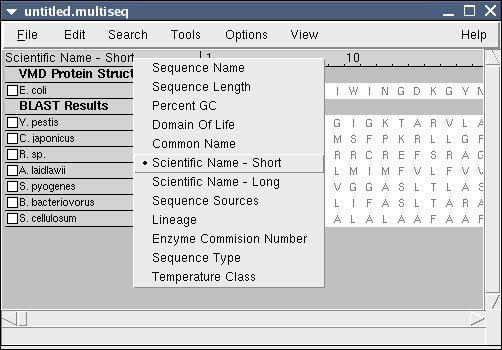
\includegraphics [width=3in]{./pictures/title_display.jpg}}
 \caption{Choosing Data To Display As Sequence Title}%more information in caption about views etc.
 \label{fig:title_display}
\end{figure}
If you choose an option where a sequence does not have a value, Multiseq
will show you the $<$Sequence Name$>$ in angle brackets.

\subsection{Grouping}
While working with the Sequence Viewer in MultiSeq, you may notice
certain patterns or trends.  As a result you would like to put certain
sequences closer to others to analyze such motifs.  MultiSeq allows such
grouping based on taxonomy or you can customize the groupings.  Right
clicking on a group name (such as \textsf{VMD Protein Structures} will bring
up a context menu where you can manage groups.

% \subsection{Managing Representations}

\subsection{Info Viewer}
Whenever you load a sequence or structure into MultiSeq an `\texttt{i}' box will
appear next to the protein's ID.  If you click on this box, a new
window will appear called the \textsf{Info Viewer} (See
Fig.~\ref{fig:editSeqInfoWindow}).  Within this window
information regarding the species the protein is from will appear. If
you have PSIPred installed and configured, you can predict the secondary
structure at the bottom of the Info window.
\begin{figure}[here]
 \centerline{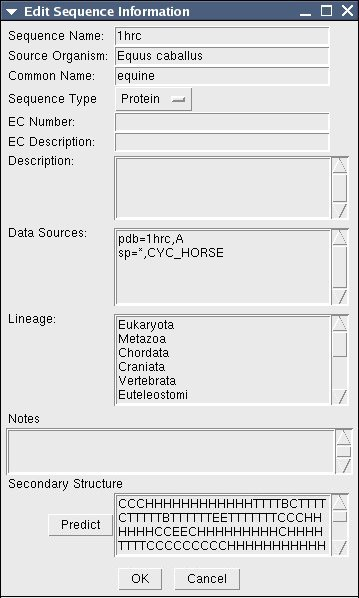
\includegraphics [width=3in]{./pictures/editSeqInfo.jpg}}
 \caption{Edit Sequence Information}%more information in caption about views etc.
 \label{fig:editSeqInfoWindow}
\end{figure}

\subsection{Selecting vs. Marking}
As you browse the menus of MultiSeq you will notice options for
\textsf{Selected Sequences} or \textsf{Marked Sequences}.  ``Selecting
Sequences'' is when you highlight a portion of the sequence(s) in the
sequence viewer using the mouse.  This can be either the entire sequence
or a portion.  However ``Marking Sequences'' allows you to more easily
select an entire sequence by simply checking the box next to the protein
ID.




